\chapter{IoT communication protocols}

IoT devices come in all shapes and sizes and used in a wide range of applications, but they share one common main goal, to collect and transmit data. Communication can either be wired or wireless, but the main concern for this kind of smart devices is the latter. Since there is no unique standard, multiple communication protocols are in use, depending on the requirements, such as, the data bandwidth, the radio range, the power consumption, the  topology or the security constraints. \\

This chapter will describe the main protocols used in IoT communications, as well as the advantages and disadvantages between them. Typically, the type of connectivity is given by the distance the data must travel, in such scenario, it is possible to divide the most common network protocols in two categories: \textit{Low-power, wide-area networks (LPWAN)} and \textit{Low-power, short-range networks} \cite{Microsoft:protocols}. The classification diagram is shown in figure \ref{fig:NetworkClassification}.


\begin{figure}[h]
    \centering
    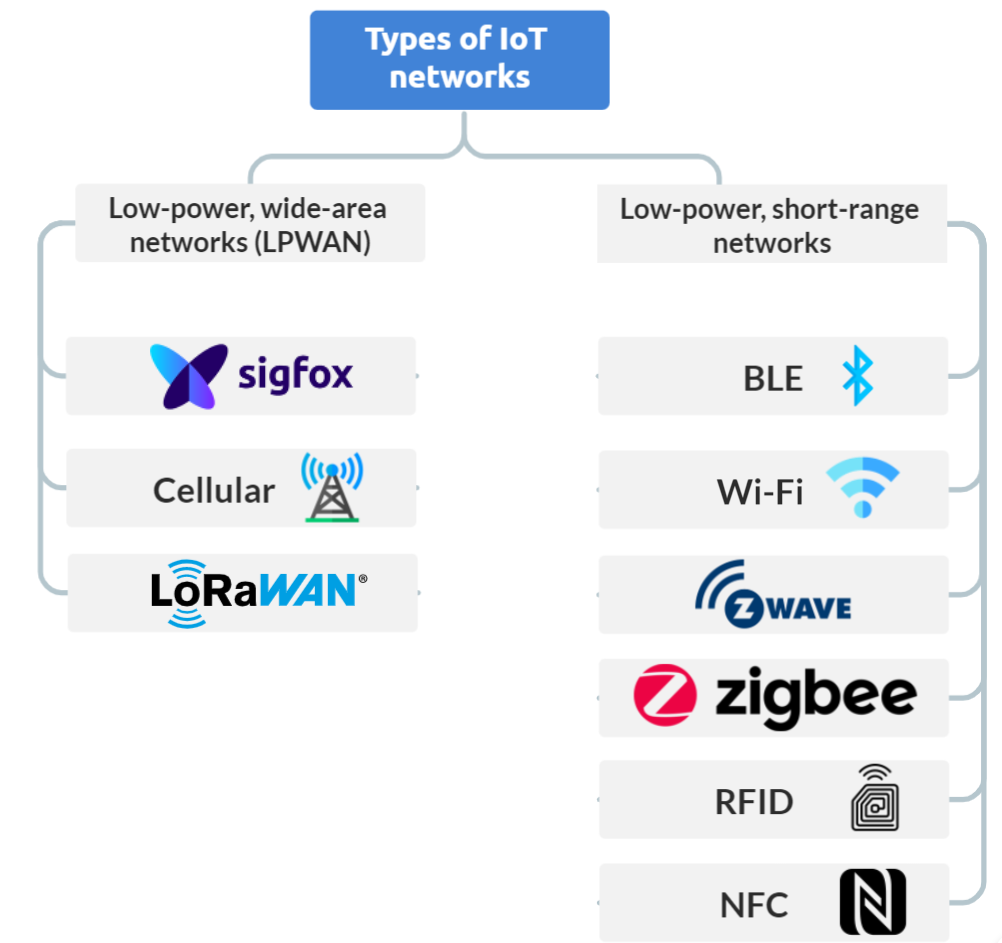
\includegraphics[width=.9\linewidth]{images/TypeOfNetworks.png}
    \caption{IoT network classification}
    \label{fig:NetworkClassification}
\end{figure}


\section{Low-power, wide-area networks (LPWAN)}
The main characteristic of LPWANs is to provide long-range communication on low-power devices. These protocols are better suited for applications that do not require high bandwidth or time-sensitive constraints \cite{BehrTech:protocols}.

\subsection{Sigfox}
The Sigfox technology is intended for M2M communication. It uses an Ultra Narrow Band channel, making data transfer speed as low as 10 to 1000 bps. On the other hand, distance between nodes can go up to 50 Km \cite{IEEE:protocols}.

\subsection{Cellular}
Although cellular networks are under the LPWAN category, they are not by any means cheap on power, on the contrary they impose high power requirements, but provide high speed communication over long distances, taking advantage of the installed GSM/3G/4G/5G mobile networks. Cellular technology is not viable for most IoT devices, since they are battery-operated.

\subsection{LoRaWAN}
The Long-Range Wide-Area Networks (LoRaWAN) is intended for transmitting small size payloads over long distances. Devices supporting this technology are optimized to operate in a low power mode, lasting up to 10 years on a single cell battery. Signals can be sent and received over a distance of 3 km in urban areas or 10 km in rural areas. The network is secured by end-to-end AES-128 encryption \cite{LoRaWAN}.

\section{Low-power, short-range networks}
This type of networks are better suited for homes, offices or small environments, since they can support short range communication, with the advantage of being inexpensive to operate and require small batteries.

\subsection{Bluetooth Low Energy (BLE)}
BLE is very significant protocol in the IoT world. According to the 2022 market report written by Bluetooth \textregistered, It is estimated that about 35\% of all IoT connected devices rely on this protocol \cite{BLE1}.
BLE was designed for short-range communications with low latency, but with low bandwidth. However it takes into account a very low power consumption. We can find devices relying on this technology in audio streaming devices, PC peripherals, accessories and fitness and health wearables. Nowadays, also very common in asset tracking and indoor navigation where GPS can not be used.

\subsection{Wi-Fi} \label{sec:wifi}
Wi-Fi technology is pretty much spread all over, including IoT applications. It provides high-throughput data transfers. However, due to its high imposing energy requirements, WiFi is not a feasible network protocol for IoT running on batteries. Instead, it is more suitable for devices that are connected to the power outlet, as security cameras or smart home appliances. The allowed distance is usually within the range of 35 m indoors and 100 m outdoors \cite{IEEE:protocols2}.

\subsection{Z-Wave}
It is a standard designed for remotely controlled residential applications, it can deliver a transmission speed of 40 kbps reaching up to 30 m. It uses AES-128 encryption for securing the channel \cite{IEEE:protocols2}.

\subsection{Zigbee}
This protocol is based on the IEEE 802.15.4 standard, it is intended for short-range low-power communications, typically deployed in mesh topologies to extend the coverage. It provides a low bit rate up to 250 kbps. It is possible to connect 65000 nodes in a single zigbee network. Operates in a rage of 10 to 100 meters 

\subsection{RFID}
Radio Frequency Identification (RFID) consists of small readers and RF tags transmitting small amount of data through radio waves within very short distances. RF tag are electronically programmed with unique information, so they cannot be used to collect measurements. However, RFID has had a great positive impact in retail and logistics, as tags can be attached to all kind of products for inventory tracking.

\subsection{NFC}
Near-Field Communication (NFC) is a protocol very similar to RFID. It can connect two devices in a distance shorter than 4 cm. It can be used for identification (similar to RFID), but also for more capable two-way communication. This technology is now extended to mobile phones, contactless payments and different industrial applications.\\

Table \ref{tab:DiffNetworks} provides a comparison between the different network protocols most used in IoT scenarios \cite{IEEE:protocols}.

\begin{table}[]
\centering
    \resizebox{\textwidth}{!}{\begin{tabular}{lccccc} 
         \hline
         Technology & Range & Data Rate & \makecell{Power \\consumption} & Topology & Security \\ 
         \hline
         Sigfox & \makecell{10 km (urban) \\ 50 km (rural)} & \makecell{100 bps (urban) \\ 600 bps (rural)} & 10 - 100 mW & Star & Custom \\ 
         Cellular & Several km & & High & - & \\ 
         LoRaWAN & < 10 km & & & & \\
         \hline
         BLE & 15 - 30 m& 1 Mbps & Low (30 mA) & Star-bus & AES-128\\
         Wi-Fi & < 100 m & & & & WPA2 \\
         Z-Wave & < 30 m & 40 kbps & Low (2.5 mA) & Mesh & AES-128 \\
         Zigbee & 10 - 100 m & 250 kbps & Low (30 mA) & Star, Mesh & AES-128 \\
         RFID & < 200 m& 4 Mbps& Ultra-low & Point-to-Point & RC4\\
         NFC & < 4 cm & 106, 212, 424 kbps& 50 mA& Point-to-Point & RSA\\
         \hline
    \end{tabular}}
    \caption{Comparison between network protocols}
    \label{tab:DiffNetworks}
\end{table}